
%=========================================================
% CONTEXTO GEOGRÁFICO
%=========================================================

El área de estudio comprende un polígono irregular dentro de la alcaldía Gustavo A. Madero. Para la delimitación espacial del análisis, se seleccionaron específicamente las Zonas Territoriales 6, 7 y 8, establecidas de manera oficial por la demarcación \cite{gam2026}.

\subsection{Delimitación de la zona de estudio}

Como se muestra en la Figura \ref{fig:mapa_zona_estudio}, las Zonas Territoriales 6, 7 y 8 reúnen una gran cantidad de lugares que generan un flujo constante de peatones. Esto se debe a la diversidad de actividades y servicios presentes en la zona, donde se encuentran hospitales, centros comerciales, espacios de entretenimiento e instituciones educativas con una gran cantidad de estudiantes. Además, estas áreas cuentan con distintas opciones de transporte público que facilitan la llegada y el desplazamiento de personas.

La combinación de estos elementos genera una importante concentración de población que se desplaza por la zona en diferentes horarios y con distintos propósitos. Debido a esta variedad de actividades, recorridos y dinámicas de movilidad, se retoman conceptos y teorías de la criminología ambiental para analizar por qué el polígono resulta adecuado para analizar el riesgo al que pueden enfrentarse los peatones.

\begin{figure}[!h]
    \centering
    \includegraphics[width=1\textwidth]{figures/capitulo3_marco_teorico/3.2_contexto_geografico/mapa.png}
    \caption{Delimitación del área de estudio propuesta (Polígono Politécnico-Vallejo). Elaboración propia en QGIS utilizando cartografía base de OpenStreetMap.}
    \label{fig:mapa_zona_estudio}
\end{figure}


\textbf{Infraestructura de transporte} \\
El polígono (especificamente la zona territorial 6 parte de la 7) es atravesado por tres sistemas de transporte público que en conjunto delimitan gran parte de su perímetro. El Sistema de Transporte Colectivo Metro concurre mediante las Líneas 3, 5 y 6: la primera bordea el flanco oriente a través de las estaciones Indios Verdes, Deportivo 18 de Marzo, Potrero y La Raza; la segunda cruza el centro del polígono conectando Politécnico, Instituto del Petróleo, Autobuses del Norte y La Raza; y la tercera enlaza Instituto del Petróleo, Lindavista y Deportivo 18 de Marzo. 

El sistema Metrobús, igual de la zona territorial 6 y parte de la zona 7 concurre mediante dos líneas que enmarcan los bordes poniente y oriente del área: la Línea 3 recorre el corredor Vallejo/Eje 1 Poniente desde Tenayuca hasta La Raza, mientras que la Línea 1 recorre Avenida Insurgentes Norte entre Indios Verdes y La Raza, coincidiendo en ambos casos con estaciones de la red de Metro antes descrita. Por otra parte, en la zona territorial 8 se encuentra una de las unidades más importantes del Instituto Politécnico Nacional: Zacatenco. En esta parte se encuentra una gran parte de transportes concesionados rodeando el area. De igual forma, esta zona tambien abarca casi toda la linea 1 cablebus (Cuautepec-Indios Verdes).

Complementariamente, el Trolebús-linea 8 (Terminal Zacatenco) opera dentro del polígono mediante la Línea 1, que conecta Autobuses del Norte, CCH Vallejo y La Raza, cuyo recorrido es interno a la Unidad Profesional Zacatenco del IPN. Véase la figura \ref{fig:todos_transportes}:\\

\begin{figure}[!h]
    \centering
    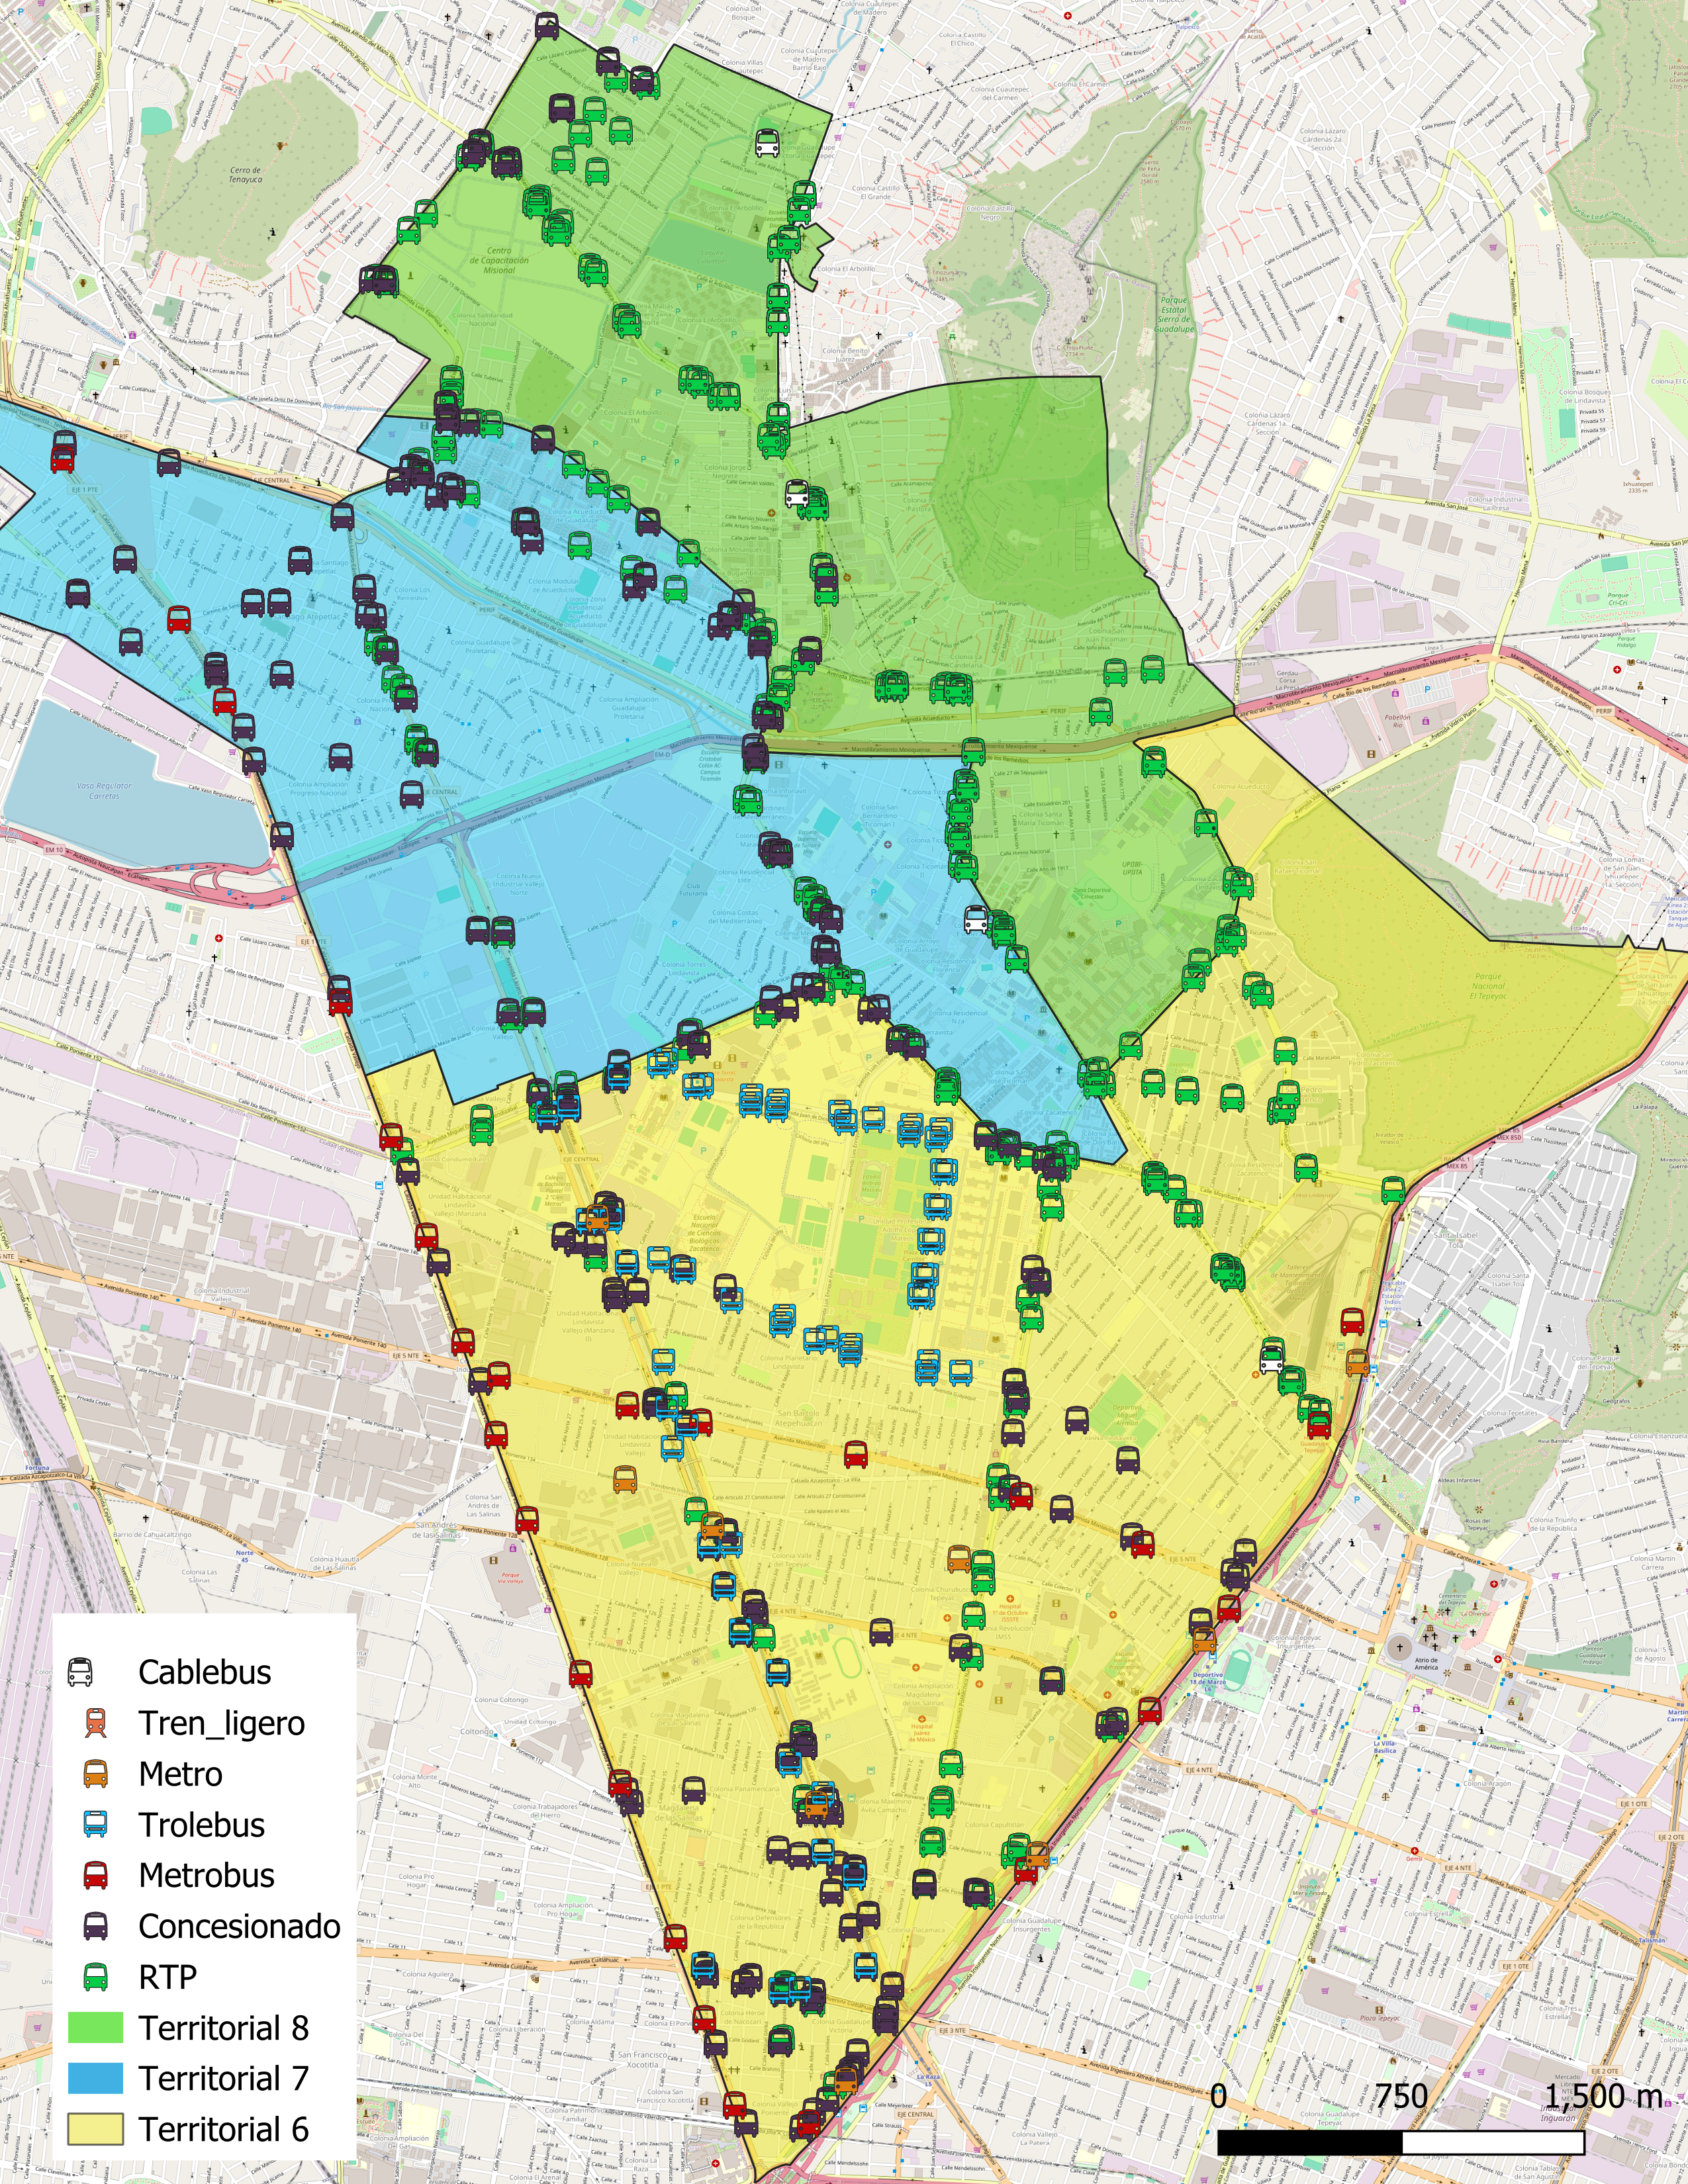
\includegraphics[width=0.8\textwidth]{figures/capitulo3_marco_teorico/3.2_contexto_geografico/transporte.png}
    \caption[Mapa integrado de la red de transporte en las Zonas Territoriales 6, 7 y 8]{Mapa integrado de la red de transporte en las Zonas Territoriales 6, 7 y 8 de la alcaldía Gustavo A. Madero. Elaboración propia mediante el software QGIS.}
    \label{fig:todos_transportes}
\end{figure}

De acuerdo con los registros de la Secretaría de Movilidad \cite{semovi_afluencia2026}, cinco de las rutas que delimitan y cruzan las Zonas Territoriales 6, 7 y 8 figuran dentro del top 18 de mayor demanda en toda la Ciudad de México. Como se detalla en el Cuadro \ref{tab:afluencia_top}, el polígono concentra a la segunda y cuarta ruta más concurridas de toda la red metropolitana (Línea 3 del Metro y Línea 1 del Metrobús). 

\begin{table}[h]
    \centering
    \caption[Afluencia de las líneas de transporte masivo en el polígono de estudio]{Afluencia de las líneas de transporte masivo en el polígono de estudio (Enero - Julio 2026) \cite{semovi_afluencia2026}.}
    
    \vspace{0.2cm}
    \begin{tabular}{|l|c|r|}
        \hline
        \textbf{Sistema y Línea} & \textbf{Lugar a nivel CDMX} & \textbf{Viajes totales} \\ \hline
        STC Metro - Línea 3 & 2$^\circ$ & 96,139,766 \\ \hline
        Metrobús - Línea 1 & 4$^\circ$ & 84,097,297 \\ \hline
        Metrobús - Línea 3 & 14$^\circ$ & 31,681,049 \\ \hline
        STC Metro - Línea 5 & 15$^\circ$ & 31,557,275 \\ \hline
        STC Metro - Línea 6 & 17$^\circ$ & 21,202,436 \\ \hline
    \end{tabular}
    \label{tab:afluencia_top}
\end{table}


Por otra parte, como se resume en el Cuadro \ref{tab:afluencia_transporte}, destaca la estación Indios Verdes con 14.7 millones de viajes en el primer semestre de 2026, cifra que la ubica de forma consistente como la tercera estación de mayor afluencia de toda la red \cite{stcmetro2026}. En contraste, Instituto del Petróleo registra el volumen más bajo del polígono, con 1.3 millones de viajes entre sus dos lineas. \cite{stcmetro2026}.


Entre enero y julio de 2026, la Línea 1 del metrobús registró 84,097,297 viajes totales, siendo la línea de mayor demanda de todo el sistema Metrobús (31\% del total de la red), mientras que la Línea 3 registró 31,681,049 viajes en el mismo periodo (11\% del total) \cite{semovi2026mb}.

En el mismo periodo, la Línea 1 del trolebús acumuló 11,841,056 viajes, mientras que la Línea 8 registró apenas 905,878 \cite{semovi2026tb}, cifra considerablemente menor que se explica por la naturaleza interna y de corta distancia de su recorrido dentro del campus.

\begin{table}[h]
\centering
\caption{Afluencia de estaciones y líneas de transporte masivo dentro del área de estudio.}
\label{tab:afluencia_transporte}
\begin{tabular}{llr}
\toprule
\textbf{Estación / Línea} & \textbf{Sistema} & \textbf{Viajes (2026)} \\
\midrule
Indios Verdes & Metro L3 & 14,743,513 \\
La Raza & Metro L3 + L5 & 6,222,363 \\
Deportivo 18 de Marzo & Metro L3 + L6 & 4,531,655 \\
Politécnico & Metro L5 & 4,288,865 \\
Autobuses del Norte & Metro L5 & 3,124,764 \\
Lindavista & Metro L6 & 2,498,111 \\
Potrero & Metro L3 & 2,180,907 \\
Vallejo & Metro L6 & 1,138,453 \\
Instituto del Petróleo & Metro L5 + L6 & 1,335,956 \\
\midrule
Línea 1 & Metrobús & 84,097,297 \\
Línea 3 & Metrobús & 31,681,049 \\
\midrule
Línea 1 & Trolebús & 11,841,056 \\
Línea 8 (Circuito Politécnico) & Trolebús & 905,878 \\
\bottomrule
\end{tabular}
\end{table}

Tener los datos aproximados de afluencia de personas en las estaciones de transporte público es importante para esta investigación porque estos espacios funcionan como nodos de actividad que concentran grandes volúmenes de desplazamientos diarios. De acuerdo con la teoría de los patrones delictivos de Brantingham y Brantingham 
\cite[p.~259-294]{brantingham1993}, la búsqueda de objetivos por parte de un delincuente y/o agresos no es aleatoria, sino que ocurre a lo largo de las rutas de tránsito habitual y en los nodos donde convergen diversas personas. En el contexto local, la evidencia confirma esta premisa; Fuentes y Sánchez \cite{fuentes2017} demostraron que las estaciones de transbordo tienen un efecto positivo estadísticamente significativo en los índices de criminalidad, estimando que un incremento del 10\% en esta variable se asocia con un aumento del 5.4\% en los robos a transeúntes. Es por esta razón por la que cuantificar la afluencia permite dimensionar e identificar las zonas de mayor exposición para los usuarios y mapear con precisión las áreas donde se requiere priorizar la seguridad.
 \\

\textbf{Zonas Industriales, Habitacionales y Escolares} \\


Como se estableció en la delimitación de la zona de estudio, el área analizada está conformada por las Zonas Territoriales 6, 7 y 8 de la alcaldía Gustavo A. Madero. Dentro de este espacio se identifican áreas industriales, habitacionales y escolares con diferentes características y funciones dentro del entorno urbano. En particular, el área de estudio no contiene extensiones de uso industrial, salvo los sectores correspondientes a Nueva Industrial Vallejo y Nueva Vallejo (Véase figura \ref{fig:uso_suelo}), mientras que sus fronteras poniente y sur colindan con corredores industriales de mayor escala. Por otra parte, el uso de suelo habitacional ocupa una parte importante del área analizada y se distribuye a lo largo de las tres Zonas Territoriales, como se observa en el mapa de uso de suelo (Figura \ref{fig:uso_suelo}). Asimismo, dentro del área de estudio se localizan diversos planteles educativos de distintos niveles, cuya distribución se muestra, de igual forma, en la Figura \ref{fig:escuelas}.

\begin{figure}[!h]
    \centering
    \includegraphics[width=0.8\textwidth]{figures/capitulo3_marco_teorico/3.2_contexto_geografico/uso_suelo.png}
    \caption[Mapa de uso de suelo: zonas habitacionales e industriales en el área de estudio]{Mapa de uso de suelo en las Zonas Territoriales 6, 7 y 8 de la alcaldía Gustavo A. Madero, destacando las áreas habitacionales y las zonas industriales (puntos morados). Elaboración propia mediante el software QGIS.}
    \label{fig:uso_suelo}
\end{figure} 

\textbf{Zonas Industriales} \\
El entorno de la zona de estudio presenta una combinación de áreas industriales que se encuentran dentro de la alcaldía Gustavo A. Madero y otros sectores industriales ubicados fuera de esta demarcación, pero que colindan directamente con el polígono de estudio. Esta distinción resulta relevante debido a que los sectores ubicados en los límites de la zona de estudio concentran puntos de acceso y conexión con el transporte público, por lo que pueden formar parte de los recorridos peatonales de las personas que se desplazan hacia o desde las áreas industriales.

Dentro de la alcaldía Gustavo A. Madero, por el flanco poniente, se encuentran Nueva Industrial Vallejo y Nueva Vallejo. La primera presenta una superficie aproximada de 1.17 km² (12,627,764.43 pies²) y una distancia total aproximada de 4.93 km (3.06 mi) \cite{googlemaps2026}. De acuerdo con los registros de la Fiscalía General de Justicia de la Ciudad de México, en este sector se documentaron 7 robos a transeúnte, 4 casos de violación, uno de ellos correspondiente a 2024, y un homicidio doloso durante 2025 \cite{FGJ2025}. Para el periodo de enero a julio de 2026 se registraron nuevamente 7 robos a transeúnte, un caso de violación y un robo a cuentahabiente \cite{FGJ2026}.

Por su parte, Nueva Vallejo cuenta con una superficie aproximada de 403,004.52 m² (4,337,904.52 pies²) y una distancia total aproximada de 3.82 km (2.37 mi) \cite{googlemaps2026}. En este sector se documentó, durante 2024, una carpeta de investigación por robo a transeúnte y una por violación \cite{FGJ2025}. Para 2025 se registraron 7 robos a transeúnte y un caso de violación \cite{FGJ2025}, mientras que durante enero-julio de 2026 se documentaron 4 carpetas por robo a transeúnte, todas tipificadas con violencia, y una denuncia adicional por violación \cite{FGJ2026}.

Fuera de la alcaldía Gustavo A. Madero, pero en contacto directo con el límite del área de estudio, se encuentran otros sectores que forman parte del entorno inmediato. En el vértice sur, el polígono colinda con Santa María Insurgentes y Atlampa, ambas ubicadas en la alcaldía Cuauhtémoc. En conjunto, estos sectores presentan una superficie aproximada de 1.59 km² (17,081,745.16 pies²) y una distancia total de 6.07 km (3.77 mi) \cite{googlemaps2026}. De acuerdo con los registros de la Fiscalía General de Justicia, durante 2025 se documentaron en este sector 13 carpetas de investigación por robo a transeúnte en vía pública, 4 casos de homicidio doloso y 2 denuncias por violación \cite{FGJ2025}. Para el periodo de enero a julio de 2026 se registraron 4 incidentes adicionales por robo a transeúnte y un caso de violación \cite{FGJ2026}.

De manera complementaria, en el entorno inmediato también se encuentra la Zona Industrial Vallejo, ubicada en la alcaldía Azcapotzalco, en colindancia con Gustavo A. Madero. Este polígono presenta una superficie aproximada de 3.76 km² (1.45 mi²) y una distancia total aproximada de 11.58 km (7.19 mi) \cite{googlemaps2026}. En 2024 se registró en este sector una carpeta por robo a transeúnte y una por violación, mientras que durante 2025 se documentaron 2 incidentes de robo a transeúnte \cite{FGJ2025}. Para enero-julio de 2026 se registraron 8 carpetas por robo a transeúnte en la vía pública, todas tipificadas con violencia, y un caso de violación \cite{FGJ2026}.

La incorporación de estos sectores externos no implica que formen parte del área de estudio, sino que permite caracterizar las condiciones existentes en sus límites y en los puntos donde se establece la conexión con el entorno urbano circundante. Esta relación resulta especialmente relevante debido a que las zonas industriales presentan una disponibilidad limitada de transporte público en su interior, por lo que los principales puntos de acceso y conexión se concentran en sus bordes \cite{googlemaps2026}. En consecuencia, las personas que se desplazan hacia estos sectores pueden realizar recorridos peatonales desde dichos puntos hasta sus lugares de trabajo, haciendo que las condiciones de las vialidades y espacios públicos ubicados en sus límites sean relevantes para el análisis.

De acuerdo con los principios de la Prevención del Delito Mediante el Diseño Ambiental (CPTED), propuesta por C. Ray Jeffrey en 1971 \cite{jeffery1971}, esta situación puede representar una mayor vulnerabilidad para los peatones. Las zonas industriales suelen presentar una configuración urbana poco diversa, en la que predominan grandes espacios destinados a una sola actividad. Es común encontrar muros extensos, fachadas con pocas ventanas y poca presencia de comercios, personas o viviendas en las calles.

Estas condiciones pueden reducir la vigilancia natural, es decir, la posibilidad de que otras personas observen lo que ocurre en el espacio público. El problema puede ser mayor fuera de los horarios de entrada y salida de los trabajadores, cuando disminuye considerablemente la cantidad de personas en las calles. Desde la perspectiva de Jeffrey, las características del entorno pueden influir en las oportunidades para cometer delitos, ya que el aislamiento y la poca interacción entre las personas facilitan que ciertas zonas sean menos visibles y transitadas.

\textbf{Zonas Habitacionales} \

El uso de suelo habitacional ocupa una parte importante de la zona de estudio y se distribuye a lo largo de las tres Zonas Territoriales, como se observa en la Figura \ref{fig:uso_suelo}. Estas áreas corresponden principalmente a espacios destinados a la residencia de la población y permiten identificar zonas en las que se concentra parte de la actividad cotidiana asociada con el ámbito doméstico.

La distribución de las zonas habitacionales resulta relevante para el análisis de movilidad debido a que pueden constituir puntos de origen de desplazamientos hacia otros espacios donde se desarrollan actividades cotidianas, como centros educativos, lugares de trabajo, comercios y otros servicios. Sin embargo, su ubicación no permite determinar por sí misma los recorridos realizados por la población, por lo que su función dentro del análisis se considera como parte de la estructura espacial a partir de la cual posteriormente se representarán posibles desplazamientos mediante el grafo de movilidad.


\textbf{Zonas Escolares} \\


De manera complementaria, el área de estudio cuenta con diversos planteles educativos distribuidos entre las tres Zonas Territoriales. Como se observa en la Figura \ref{fig:escuelas}, se identifican instituciones de distintos niveles educativos. Entre estas instituciones destaca la presencia de instalaciones del Instituto Politécnico Nacional.

\begin{figure}[!h]
    \centering
    \includegraphics[width=0.8\textwidth]{figures/capitulo3_marco_teorico/3.2_contexto_geografico/escuelas.png}
    \caption[Escuelas de nivel superior, medio superior, secundarias y básicas]{Mapa de escuelas de nivel superior, medio superior, secundarias y básicas en las Zonas Territoriales 6, 7 y 8 de la alcaldía Gustavo A. Madero. Elaboración propia mediante el software QGIS.}
    \label{fig:escuelas}
\end{figure}

La presencia de instituciones educativas permite identificar espacios en los que se desarrollan actividades recurrentes de la población, particularmente aquellas relacionadas con la formación académica. Su distribución dentro del área de estudio resulta relevante para el análisis de movilidad debido a que estos espacios pueden constituir destinos frecuentes para estudiantes, docentes y personal administrativo.

La importancia de las instituciones educativas dentro del área de estudio puede observarse particularmente en el caso del Instituto Politécnico Nacional. De acuerdo con Data México, en 2022 el IPN registró 128,869 estudiantes matriculados en la Ciudad de México, mientras que 56,450 correspondieron a Gustavo A. Madero \cite{datamexico_ipn}. Estos datos permiten dimensionar la presencia de la institución en la demarcación. Además, el propio IPN señala que en la Unidad Profesional ``Adolfo López Mateos'' convergen diariamente más de 30 mil alumnos y 5 mil docentes e investigadores en un área aproximada de 2.5 kilómetros de largo por 2.5 kilómetros de ancho\cite{ipn2022}.

\textbf{Las actividades rutinarias como punto de partida} \

La distribución conjunta de las zonas habitacionales, escolares e industriales puede analizarse a partir de la teoría de las actividades rutinarias propuesta por Cohen y Felson. Los autores definen las actividades rutinarias como aquellas actividades recurrentes y habituales que forman parte de la vida cotidiana y permiten cubrir distintas necesidades de la población, como el trabajo, la obtención de alimentos, el ocio y la interacción social \cite{cohenfelson1979}. Estas actividades se desarrollan en diferentes lugares, por lo que pueden generar desplazamientos entre los espacios donde las personas residen y aquellos donde realizan sus actividades cotidianas.

Desde esta perspectiva, las zonas habitacionales pueden representar posibles puntos de origen, mientras que las instituciones educativas y las áreas industriales pueden corresponder a espacios vinculados con actividades que generan desplazamientos recurrentes. En particular, los sectores industriales constituyen espacios relacionados con actividades laborales, mientras que las instituciones educativas concentran actividades académicas que se desarrollan de manera periódica. La ubicación de estos elementos permite, por tanto, identificar relaciones espaciales entre lugares de residencia y algunos de los posibles destinos asociados con las actividades cotidianas, sin asumir de antemano los recorridos que realizan las personas.

Estos datos no permiten determinar por sí mismos los recorridos realizados por estudiantes, docentes, trabajadores o residentes, pero sí muestran la existencia de espacios con diferentes concentraciones y tipos de actividad cotidiana. De acuerdo con Cohen y Felson, la distribución de estas actividades fuera del hogar puede generar la convergencia de personas en determinados lugares y momentos, modificando las oportunidades para la ocurrencia de delitos \cite{cohenfelson1979}. En este sentido, la oportunidad constituye un elemento relevante para analizar la relación entre las actividades cotidianas, la movilidad y el delito \cite{canopanos2018}.

Por lo tanto, las zonas habitacionales, escolares e industriales no se consideran por sí mismas como espacios de mayor o menor riesgo. Su inclusión en el análisis responde a su relación con las actividades cotidianas de la población y a su posible función como puntos de origen o destino dentro de los desplazamientos que serán representados mediante el grafo de movilidad.


\subsubsection{Síntesis del contexto geográfico}

El análisis realizado permite identificar que las Zonas Territoriales 6, 7 y 8 presentan una combinación de espacios asociados con distintas actividades y desplazamientos cotidianos. En el área de estudio se encuentran zonas habitacionales, instituciones educativas, zonas industriales y una red de transporte público, cuya distribución permite caracterizar parte de las condiciones espaciales en las que se desarrollan las actividades de la población.

Esta configuración puede interpretarse a partir de la teoría de las actividades rutinarias, ya que las actividades cotidianas se desarrollan en distintos lugares y pueden generar desplazamientos entre ellos \cite{cohenfelson1979}. Desde esta perspectiva, la distribución de los espacios habitacionales, educativos e industriales permite identificar posibles relaciones entre lugares de residencia y destinos asociados con actividades cotidianas, mientras que la red de transporte constituye parte de la infraestructura mediante la cual se realizan estos desplazamientos.

A su vez, las características físicas de determinados espacios, particularmente de las zonas industriales, permiten incorporar elementos de la Prevención del Delito Mediante el Diseño Ambiental. Aspectos como el aislamiento, la configuración de los espacios y las condiciones de vigilancia natural pueden ser considerados dentro del análisis del entorno construido. Estos elementos se complementan con los registros oficiales de delitos y la información disponible sobre percepción de inseguridad, considerando que las estadísticas delictivas no representan la totalidad de los hechos ocurridos debido a la existencia de una cifra negra.

En conjunto, esta información permite caracterizar el contexto geográfico de la zona de estudio y establecer los elementos que serán considerados en el análisis posterior. A partir de la distribución de los distintos tipos de espacios y de la red vial, se construirá el grafo de movilidad, en el que las vialidades y sus conexiones constituirán la base para representar los desplazamientos peatonales. Posteriormente, los factores identificados en el contexto geográfico y los registros de delito serán incorporados al análisis de los tramos de la red para determinar los componentes que intervienen en el cálculo del costo de desplazamiento y, finalmente, en la generación de rutas peatonales.
